% =============================================================================
% Connect-4 Reinforcement Learning - Project 3 Report
% Optimization II, UT Austin MSBA, Spring 2026
%
% This file is the skeleton. Paste the whole thing into Overleaf, then iterate
% section by section. All figures should live in report/figures/ and can be
% referenced by filename alone thanks to \graphicspath below.
% =============================================================================

\documentclass[11pt]{article}

% ── Packages ─────────────────────────────────────────────────────────────────
\usepackage[margin=1in]{geometry}
\usepackage{graphicx}          % figures
\usepackage{booktabs}          % nicer tables (\toprule, \midrule, \bottomrule)
\usepackage{amsmath, amssymb}  % math
\usepackage{hyperref}          % clickable refs and URLs
\usepackage{caption}
\usepackage{subcaption}
\usepackage{parskip}           % space between paragraphs, no first-line indent

% Figures live in the figures/ subfolder; use \includegraphics{name.png} only.
\graphicspath{{figures/}}

% ── Title block ──────────────────────────────────────────────────────────────
\title{%
  Connect-4 Reinforcement Learning: \\
  \large Comparing Policy Gradient and Deep Q-Network Agents
}
\author{%
  Stiles Clements \quad Alina Hota \quad Luke Hartfield \quad Zan Merrill \\[0.6em]
  \normalsize MSBA 2026 Optimization II - Project 3
}
\date{\today}

\begin{document}
\maketitle

% ── Executive summary ────────────────────────────────────────────────────────
\begin{abstract}
We piloted reinforcement learning as a way to produce stronger
single-player Connect-4 opponents than hand-written rules or
supervised imitation can generate alone. Starting from six supervised
networks that imitated Monte-Carlo tree-search decisions, we
implemented and compared two paradigms covered in this course: a
policy gradient agent that directly optimises a column-distribution
network through discounted-return-weighted log-probability gradients,
and a Deep Q-Network agent that learns a state--action value function
through a Double-DQN target with a replay buffer, target-network
synchronisation, and curriculum self-play. On a shared evaluation
harness, the policy gradient agent reached a $60.8\%$ mean win rate
while the Deep Q-Network agent reached $76.2\%$ --- $+15.4$~percentage
points stronger and the strongest agent we trained. A Soft
Actor-Critic extension that fuses the two paradigms reached $75.5\%$,
comparable to the Deep Q-Network and confirming that the off-policy
actor-critic approach is competitive with the strongest
discrete-action method.

We recommend hiring one reinforcement learning specialist for a 3--6
month engagement to build an AlphaZero-style agent (a learned policy
plus value network combined with Monte-Carlo tree search at inference
time) on top of the codebase developed for this pilot. Self-play
already produces an opponent substantially stronger than the
supervised baselines we started from; closing the remaining gap to
expert play most directly requires tree-search techniques that benefit
from dedicated reinforcement-learning expertise.
\end{abstract}

% ── 1. Introduction ──────────────────────────────────────────────────────────
\section{Introduction}
\label{sec:intro}

Our company is evaluating reinforcement learning as a technique for
generating strong computer opponents in single-player modes of our board
games. Today our opponents are rule-based, which caps opponent quality at
whatever heuristics a designer can hand-write; reinforcement learning
promises agents that \emph{learn} to play, and can keep improving with more
compute. Before committing engineering resources, we wanted a concrete pilot
on a game simple enough to prototype end-to-end in a few weeks but
non-trivial enough that the results would generalize. We chose Connect-4.

Connect-4 is a good pilot for three reasons. First, it is \emph{solved} (Allis,
1988): the first player wins with perfect play, so we have a well-defined
ceiling for any agent. Second, it is small: only seven legal moves from any
position, which makes training loops cheap and makes full-game simulations
feasible inside a reinforcement learning inner loop. Third, it closely
resembles in structure the games we actually sell (turn-based, perfect
information, discrete action space), so lessons transfer.

This report covers two reinforcement learning paradigms we implemented and
compared. Policy gradient (Section~\ref{ssec:pg} and
Section~\ref{sec:results}) directly optimizes a policy network
$\pi_\theta(a \mid s)$ that outputs a probability distribution over moves:
each parameter update is taken in the direction of the estimated gradient
$\nabla_\theta \mathbb{E}_{\tau \sim \pi_\theta}\!\bigl[R(\tau)\bigr]$ of the
expected return $R(\tau)$ over trajectories $\tau$. Deep Q-Network
(Section~\ref{ssec:dqn}) instead learns a state-action value function
$Q_\theta(s, a)$ that estimates the discounted return of playing column $a$
in position $s$ and following a greedy policy thereafter; moves at play time
are chosen as $\arg\max_a Q_\theta(s, a)$ over legal columns. Both agents are
trained by self-play against a growing pool of opponents that includes
supervised baseline networks from a previous project plus frozen snapshots
of the improving agent itself. We measure performance by win rate against
shared baseline opponents and by head-to-head play between the two agents.

The central questions this report answers for the reader are the following.
(1) Does self-play reinforcement learning produce a meaningfully stronger
Connect-4 agent than the supervised baselines we started from?
(2) Which of policy gradient or Deep Q-Network is the better investment for
our use case?
(3) Is it worth hiring dedicated reinforcement learning expertise to pursue
this further?

% ── 2. Methodology ───────────────────────────────────────────────────────────
\section{Methodology}
\label{sec:method}

\subsection{Board representation and game engine}
\label{ssec:engine}

All game logic operates on a canonical board: a $6 \times 7$ integer array
where $+1$ denotes a piece belonging to the first player (red), $-1$ denotes
the second player (yellow), and $0$ denotes an empty cell. Row~0 is the top
of the board; row~5 is the bottom. A dropped piece falls to the
highest-numbered empty row in its column, matching standard Connect-4 rules.

Our engine exposes the primitives that the training loops need:
\texttt{legal\_moves} returns the set of non-full columns;
\texttt{make\_move} applies a move and returns a new board;
\texttt{is\_terminal} detects win, loss, or draw states; and
\texttt{winning\_move}/\texttt{blocking\_move} look one ply ahead for
immediate tactical moves. The last two are used to strengthen opponent
behaviour (see Section~\ref{ssec:pg}); the agent under training never uses
them, so it is forced to learn tactics through gradient descent rather than
inherit them from hand-written rules.

Because the supervised networks we inherited from a prior project were
trained on slightly different input encodings, our \texttt{model\_loader}
module wraps every network and exposes a single
\texttt{predict\_probs(board, player)} interface. Internally it converts
the canonical board into whichever encoding the underlying network
expects: a single-channel signed representation (Type~A), a two-channel
one-hot per-player representation (Type~B), or a flattened variant of
Type~B used by one of the Transformer networks. This abstraction keeps
every other module in the codebase encoding-agnostic.

\subsection{Starting models}
\label{ssec:start}

Three teammate groups (anonymised here as Groups~A, B, and~C) each
contributed two supervised networks from a prior project, trained to
mimic Monte-Carlo tree search decisions: one convolutional network and
one Transformer per group, for six networks in total — labelled CNN-A
through CNN-C and Transformer-A through Transformer-C. We designated
Transformer-A as $M_1$, the agent we would improve via reinforcement
learning. The remaining five networks plus the original (frozen) copy
of Transformer-A formed the initial opponent pool. Per the assignment's
requirements, these original networks are never removed from the pool
during training.

\subsection{Policy gradient self-play}
\label{ssec:pg}

Our policy gradient procedure trains $M_1$ over many \emph{groups} of
self-play games. Each group proceeds as follows.

\begin{enumerate}
    \item Sample an opponent $M_2$ uniformly at random from the current
    opponent pool.

    \item Play $n_\text{games}$ games of $M_1$ versus $M_2$. For each game,
    the side $M_1$ plays (red or yellow) is chosen by drawing uniformly from
    $\{+1, -1\}$, and a small number of moves at the start are played
    uniformly at random by both sides to diversify the positions the agent
    encounters.

    \item On every $M_1$ turn after the warm-up, we sample a move
    stochastically from the masked, renormalized policy output. If
    $\mathcal{L}(s) \subseteq \{0, 1, \ldots, 6\}$ is the set of legal
    columns in board state $s$ and $\pi_\theta(a \mid s)$ is the raw
    policy-network output, we define the masked policy
    \[
        \tilde{\pi}_\theta(a \mid s)
        \;=\;
        \frac{\pi_\theta(a \mid s) \cdot \mathbf{1}\!\bigl[a \in \mathcal{L}(s)\bigr]}
             {\sum_{a' \in \mathcal{L}(s)} \pi_\theta(a' \mid s)}
    \]
    and draw the move as $a_t \sim \tilde{\pi}_\theta(\cdot \mid s_t)$.
    Stochastic sampling, rather than $\arg\max$ selection, is what provides
    the exploration signal that the policy gradient estimator relies on.

    \item For every $M_1$ move in a completed game, we record the board state
    $s_t$, the chosen column $a_t$, and the discounted return from the
    terminal outcome,
    \[
        G_t \;=\; r \cdot \gamma^{N - 1 - t},
    \]
    where $r \in \{+1, 0, -1\}$ is the game outcome from $M_1$'s perspective
    (win, draw, loss), $N$ is the number of $M_1$ moves in that game, and
    $\gamma \in (0, 1]$ is the discount factor. This weighting assigns
    higher credit to moves closer to the end of the game.

    \item After a fixed number of games we sample a fixed-size mini-batch
    $\mathcal{B}$ of triplets $(s_t, a_t, G_t)$ and take a single gradient
    descent step on the policy gradient objective
    \[
        \mathcal{L}(\theta)
        \;=\;
        -\,\frac{1}{|\mathcal{B}|}
        \sum_{(s_t, a_t, G_t) \in \mathcal{B}}
            G_t \cdot \log \tilde{\pi}_\theta(a_t \mid s_t)
        \;-\; \beta \, \mathcal{H}\!\bigl(\tilde{\pi}_\theta(\cdot \mid s_t)\bigr),
    \]
    where
    $\mathcal{H}\!\bigl(\tilde{\pi}_\theta(\cdot \mid s_t)\bigr)
     = -\sum_{a} \tilde{\pi}_\theta(a \mid s_t) \log \tilde{\pi}_\theta(a \mid s_t)$
    is the entropy of the masked policy at $s_t$ and $\beta \geq 0$ is its
    coefficient. The entropy term discourages the policy from collapsing to
    a handful of moves; we anneal $\beta$ linearly from a positive starting
    value $\beta_0$ down to zero,
    \[
        \beta(g) \;=\; \beta_0 \cdot \Bigl(1 - \tfrac{g - 1}{G - 1}\Bigr),
    \]
    where $g$ is the current group and $G$ is the total number of groups, so
    the policy can sharpen in the late stage of training. The parameter
    update is
    \[
        \theta \;\leftarrow\; \theta - \eta \, \nabla_\theta \mathcal{L}(\theta),
    \]
    where $\eta$ is the learning rate.

    \item Periodically, a frozen copy of $M_1$'s current weights is added to
    the opponent pool. This enforces self-play against a moving target: as
    the agent improves, the pool slowly accumulates stronger versions of
    itself while never removing the original supervised networks.
\end{enumerate}

Opponents are treated slightly asymmetrically. When $M_2$'s turn arrives we
first check for immediate tactical moves: if $M_2$ can win in a single move
we play that column; if $M_1$ would win on its next move we play the column
that blocks it. Only if neither shortcut applies do we sample from $M_2$'s
masked policy. $M_1$ has no such shortcut. This adversarial setup pushes
$M_1$ to learn structure that outplays a one-move-lookahead opponent rather
than winning cheaply by exploiting opponents that miss obvious threats.

\subsection{Deep Q-Network}
\label{ssec:dqn}

Our Deep Q-Network agent uses the same convolutional feature extractor as the
policy gradient network but replaces the softmax output with a linear layer
that emits a value $Q_\theta(s, a)$ for each of the seven columns. Actions
are selected with an $\epsilon$-greedy policy over the legal columns,
\[
    a_t \;=\;
    \begin{cases}
        \text{uniform}\bigl(\mathcal{L}(s_t)\bigr) & \text{with probability } \epsilon, \\[0.2em]
        \displaystyle \arg\max_{a \in \mathcal{L}(s_t)} Q_\theta(s_t, a) & \text{with probability } 1 - \epsilon,
    \end{cases}
\]
where the exploration rate $\epsilon$ is annealed from $1.0$ at the start of
training down to a small terminal value $\epsilon_\text{end}$.

Transitions are stored in a replay buffer $\mathcal{D}$ as tuples
$(s_t, a_t, r_t, s_{t+1}, d_t)$, where $s_{t+1}$ is the board at the agent's
\emph{next} turn after the opponent has moved (matching the coin-game
framing from class rather than storing the post-agent-move board), and
$d_t \in \{0, 1\}$ indicates whether $s_{t+1}$ is terminal. Training
minimises the squared Double Deep Q-Network (van Hasselt et al., 2016)
temporal-difference error
\[
    \mathcal{L}(\theta)
    \;=\;
    \mathbb{E}_{(s_t, a_t, r_t, s_{t+1}, d_t) \,\sim\, \mathcal{D}}
    \Bigl[\bigl(y_t - Q_\theta(s_t, a_t)\bigr)^{2}\Bigr],
\]
with the bootstrapped target
\[
    y_t
    \;=\;
    r_t
    \;+\;
    (1 - d_t)\, \gamma \cdot
    Q_{\theta^{-}}\!\Bigl(
        s_{t+1},\,
        \arg\max_{a \in \mathcal{L}(s_{t+1})} Q_\theta(s_{t+1}, a)
    \Bigr),
\]
where the online network $Q_\theta$ chooses the bootstrap action and the
target network $Q_{\theta^{-}}$ evaluates it. The target-network weights are
refreshed as $\theta^{-} \leftarrow \theta$ every fixed number of training
steps. This combination of a replay buffer, a target network,
$\epsilon$-annealing, and Double Deep Q-Network targets is standard for
stabilising value-based deep reinforcement learning.

To match the policy gradient setup, the Deep Q-Network agent is trained
against opponents drawn uniformly from the same pool of supervised networks.
To avoid many games that end on move three and provide no meaningful
learning signal, each game is initialised with a small number of uniformly
random moves before the agent takes over; those random moves are not
inserted as transitions into $\mathcal{D}$.

\subsection{Soft Actor-Critic extension}
\label{ssec:sac}

In addition to the policy gradient and Deep Q-Network agents that form
this report's primary comparison, we implemented a Soft Actor-Critic
agent in its discrete-action form as an
extension. Soft Actor-Critic is a natural fusion of the two paradigms
covered in this course: it trains a policy network $\pi_\phi(a \mid s)$
by gradient descent on log-probabilities (the policy gradient side) and
a state-action value network $Q_\theta(s, a)$ by temporal-difference
bootstrapping with a slowly-updated target network (the $Q$-learning
side). The motivation was practical: vanilla policy gradient suffered
from high gradient variance under Connect-4's sparse $\pm 1$ reward and
from catastrophic forgetting once $M_1$ outgrew most of the opponent
pool, and an intermediate Actor-Critic implementation reduced the
variance but remained on-policy and sample-inefficient.

Soft Actor-Critic is off-policy: transitions are stored in a replay
buffer $\mathcal{D}$ and reused across many gradient steps. The policy
is regularised toward stochasticity by adding an entropy bonus to the
Bellman backup. Concretely, the $Q$-network minimises an $n$-step soft
temporal-difference error,
\[
    \mathcal{L}_Q(\theta)
    \;=\;
    \mathbb{E}_{(s, a, r, s', d) \,\sim\, \mathcal{D}}
    \!\left[
    \Bigl(
    Q_\theta(s, a)
    \;-\;
    \bigl(r + \gamma^{n}(1 - d)\, V_{\theta^{-}}(s')\bigr)
    \Bigr)^{\!2}
    \right],
\]
where the soft state-value is computed from the target $Q$-network
$Q_{\theta^{-}}$ as
\[
    V_{\theta^{-}}(s')
    \;=\;
    \sum_{a'} \pi_\phi(a' \mid s')\,
    \Bigl[\,
    Q_{\theta^{-}}(s', a')
    \;-\;
    \alpha \log \pi_\phi(a' \mid s')
    \,\Bigr].
\]
The policy network is updated to minimise
\[
    \mathcal{L}_\pi(\phi)
    \;=\;
    \mathbb{E}_{s \sim \mathcal{D}}
    \!\left[
    \sum_{a} \pi_\phi(a \mid s)
    \Bigl(
    \alpha \log \pi_\phi(a \mid s)
    \;-\;
    Q_\theta(s, a)
    \Bigr)
    \right].
\]
Compared to the standard Bellman backup of Section~\ref{ssec:dqn}, the
$\max$ over actions has been replaced by a soft maximum that includes
an entropy bonus $-\alpha \log \pi_\phi(a \mid s)$. The temperature
$\alpha$ controls how strongly the policy is pushed toward
stochasticity: as $\alpha \to 0$ the backup recovers the hard $\max$ of
standard $Q$-learning, and as $\alpha \to \infty$ the policy collapses
toward uniform. The target network is updated by Polyak averaging
$\theta^{-} \leftarrow \tau\,\theta + (1 - \tau)\,\theta^{-}$ with a
small mixing coefficient $\tau$, so the bootstrap target drifts slowly
and does not chase its own tail.

Three project-specific choices proved important. First, the policy
network was warm-started from CNN-C rather than from random
initialisation: its seven-column softmax head was preserved, the
$Q$-head was randomly initialised, and the two heads share a trunk.
This started training near the supervised baseline of CNN-C rather
than at chance. Second, the
temporal-difference target uses an $n$-step return with $n = 3$, which
propagates credit faster than one-step TD without incurring the
variance of full Monte-Carlo returns. Third, every transition added to
the replay buffer is also added in horizontally-mirrored form,
exploiting Connect-4's reflection symmetry to roughly double the
effective sample size at negligible compute cost. A small reward-shaping
signal proportional to the change in net open-three threats was added
at each step with coefficient $0.03$, kept weak enough that it could
not overwhelm the terminal $\pm 1$ outcome.

Final hyperparameters are listed in Table~\ref{tab:sac_hparams}. The
two most sensitive were the entropy temperature $\alpha$ and the
bootstrap horizon $n$: $\alpha = 0.1$ kept the late-training policy
too soft and capped mean win rate near $70\%$, while $\alpha = 0.03$
allowed the policy to sharpen on strong moves while preserving
exploration.

\begin{table}[h]
  \centering
  \begin{tabular}{lrl}
    \toprule
    Hyperparameter                          & Value      & Notes \\
    \midrule
    Entropy temperature $\alpha$            & $0.03$     & balances exploration vs.\ sharpness \\
    Bootstrap horizon $n$                   & $3$        & faster credit than 1-step, lower variance than 5 \\
    Target update rate $\tau$               & $0.005$    & standard Soft Actor-Critic default \\
    Replay buffer capacity                  & $50{,}000$ & approximately $1{,}000$ games of transitions \\
    Batch size                              & $128$      & held constant across all updates \\
    Reward shaping coefficient              & $0.03$     & per net-open-three-threat change \\
    Originals-to-snapshots pool weight      & $3 : 1$    & prevents drift onto self-copies \\
    Tactical-opponent probability           & $0.5$      & half of $M_2$'s games use one-ply tactics \\
    \bottomrule
  \end{tabular}
  \caption{Final hyperparameters for the Soft Actor-Critic agent.}
  \label{tab:sac_hparams}
\end{table}

\subsection{Evaluation protocol}
\label{ssec:eval}

To compare agents fairly we use a shared evaluation harness. For each
pairing we play $N$ games and alternate which agent moves first so any
first-player advantage is averaged out. We report win rate, draw rate, and
average game length. Baselines include the original supervised networks, a
uniformly random policy, and depth-limited minimax at search depths of~3
and~5 as calibrated strength references. Unlike the training loops,
evaluation selects the policy gradient move as
$\arg\max_{a \in \mathcal{L}(s)} \pi_\theta(a \mid s)$ and the Deep Q-Network
move as $\arg\max_{a \in \mathcal{L}(s)} Q_\theta(s, a)$, because at
deployment we want the strongest move rather than a sample.

% ── 3. Results ───────────────────────────────────────────────────────────────
\section{Results}
\label{sec:results}

\subsection{Policy gradient training}

% ── TODO: PG experiment notes go here. The figure is already wired up below.
% Things to cover:
%   - Starting win rate and where it ended up
%   - Key hyperparameters you settled on (LR, gamma, batch size, entropy coeff)
%   - What experiments you tried and what happened (e.g. different LR, entropy annealing)
%   - Why you think it plateaued where it did

\begin{figure}[h]
  \centering
  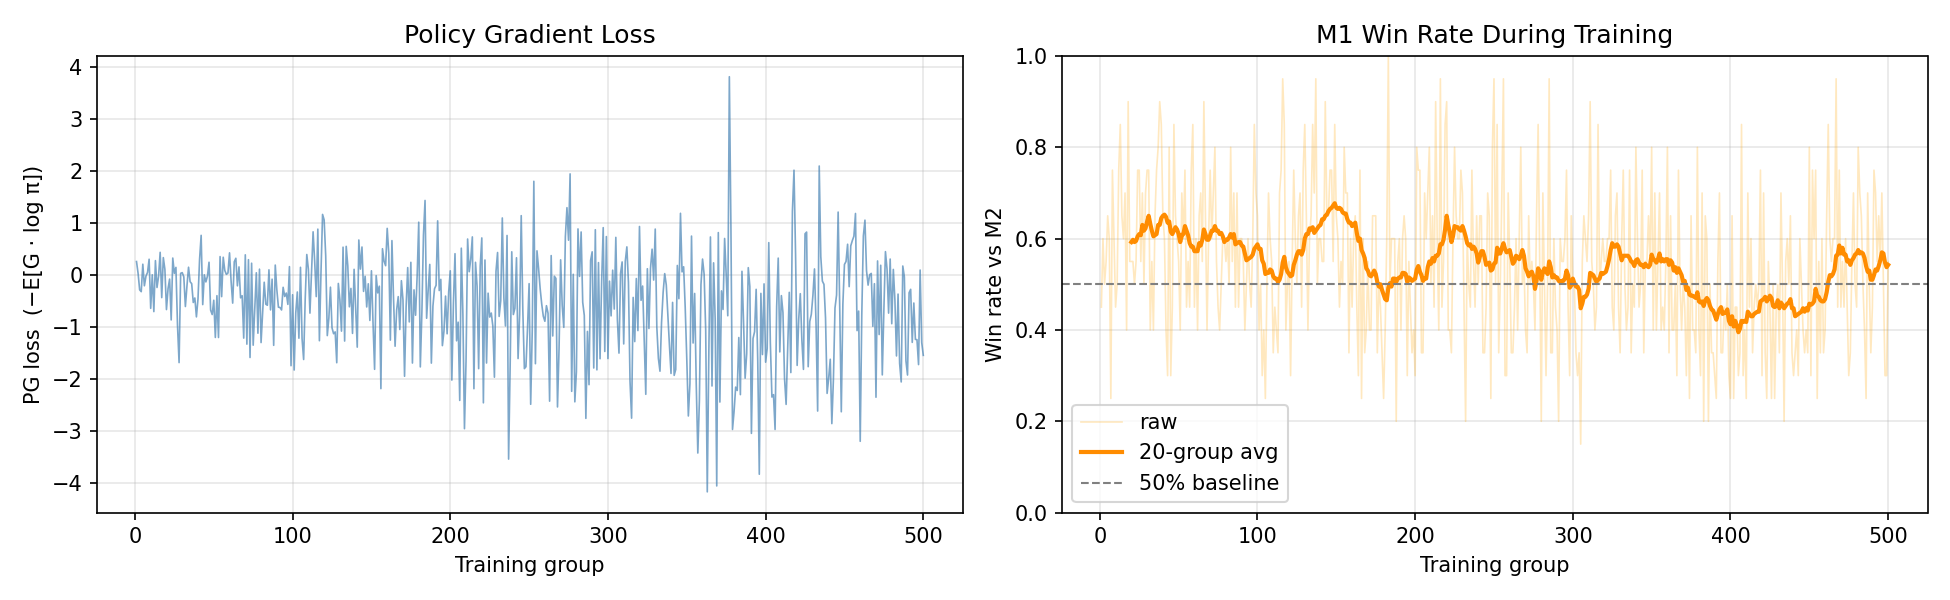
\includegraphics[width=0.95\textwidth]{pg_training_curves.png}
  \caption{Policy gradient training over 500 groups. Left: policy loss
  (negative log-likelihood weighted by discounted return). Right: M1 win rate
  against a uniformly-sampled opponent pool; the 20-group smoothed average
  (orange) rises from roughly 40\% to a plateau near 60\%. The dashed line
  marks the 50\% baseline.}
  \label{fig:pg_training}
\end{figure}

\subsection{Deep Q-Network training}
\label{ssec:dqn_results}

We trained the DQN through three successive versions, each addressing
concrete weaknesses identified in the previous run.

\textbf{Version~1} served as a proof of concept. It used a basic CNN
Q-network, a \texttt{deque}-backed replay buffer (whose \texttt{list()}
conversion made each sample an $O(n)$ operation), and no compiled
training graph. With only 50~episodes of 30~games each, it failed to
reach the 60.8\% policy-gradient baseline on shared evaluation
opponents.

\textbf{Version~2} was a full redesign. We replaced the replay buffer
with a pre-allocated \texttt{numpy} circular array (O(1) sampling),
compiled the Double-DQN training step with \texttt{@tf.function}
(reducing wall time from $\approx$28\,s per episode to $<$2\,s), and
switched to the Dueling DQN architecture described in
Section~\ref{ssec:dqn}. We also introduced a self-play pool of up to
10~frozen weight snapshots and dense intermediate rewards for creating
or eliminating three-in-a-row threats. Training ran for
400~episodes $\times$ 50~games (20{,}000~games total) in 90.6~minutes
on a Colab T4 GPU. Final evaluation against fixed opponents (greedy
play, $\epsilon=0$) yielded \textbf{81.5\%} vs.\ a random policy and
\textbf{69.5\%} vs.\ the 1-ply heuristic, for a \textbf{75.5\%}
average --- a +14.7 percentage point improvement over the PG baseline.
Win rate against its own self-play snapshots was 42\%, indicating the
agent had learned to exploit weaker opponents well but was not yet
robust against itself.

\textbf{Version~3} addressed the remaining bottlenecks. We added
$n$-step returns ($n=3$), which accumulate three steps of discounted
reward before bootstrapping from the target network, giving the network
a stronger gradient signal when a win is two or three moves away rather
than requiring three sequential TD updates to propagate the win
backward. We also compiled frozen opponent inference with
\texttt{@tf.function}, cutting self-play simulation from $\approx$18\,s
to $\approx$3\,s per episode, and applied cosine learning-rate decay
($3\times10^{-4}\to10^{-5}$) to prevent the loss from oscillating at
the flat plateau we observed in v2. These changes allowed 700~episodes
(35{,}000~games, 139{,}000 gradient steps) in 103.7~minutes while
keeping per-episode wall time at 8.9\,s on average.

The v4 evaluation results are reported in Table~\ref{tab:dqn_progression}
and Figure~\ref{fig:dqn_training}.

\begin{table}[h]
  \centering
  \begin{tabular}{lrrrr}
    \toprule
    Version & vs Random & vs Heuristic & vs Self-play & Average \\
    \midrule
    DQN v1  & $<$60\%   & $<$60\%      & ---          & $<$60\%  \\
    DQN v2  & 81.5\%    & 69.5\%       & 42.0\%       & 75.5\%   \\
    DQN v3  & 73.0\%    & 72.0\%       & 71.0\%       & 72.5\%   \\
    DQN v4  & \textbf{82.0\%} & 70.5\%  & 65.5\%       & \textbf{76.2\%} \\
    \midrule
    PG (baseline) & \multicolumn{3}{c}{---} & 60.8\% \\
    \bottomrule
  \end{tabular}
  \caption{DQN win rates across training versions (greedy play, 200~games
  each). All versions beat the PG baseline. v4 uses curriculum self-play
  (20\%--50\% self-play fraction) and resumes from v3 weights.}
  \label{tab:dqn_progression}
\end{table}

\begin{figure}[h]
  \centering
  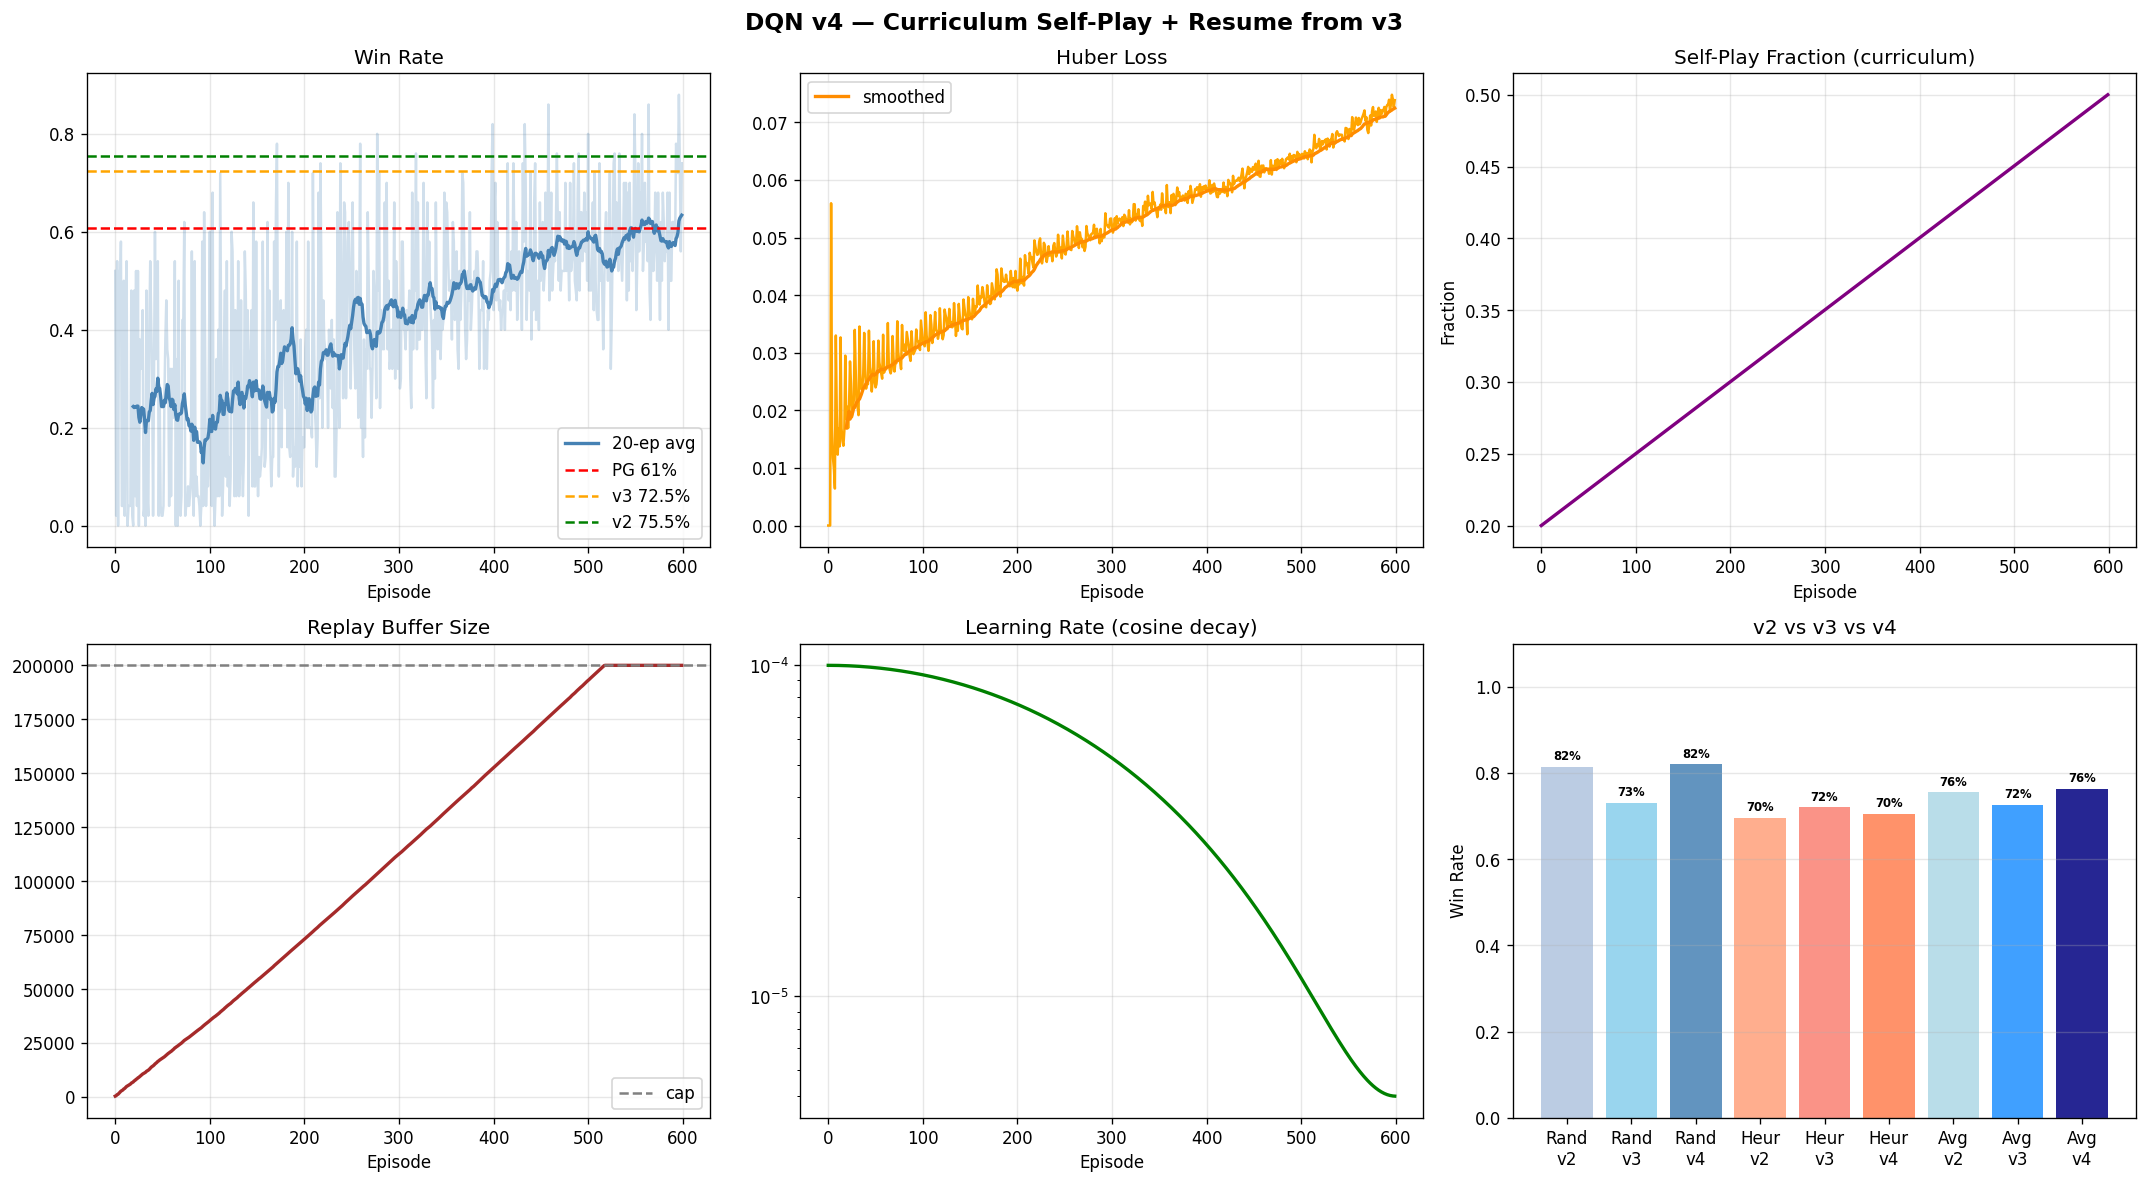
\includegraphics[width=0.95\textwidth]{dqn_v4_curves.png}
  \caption{DQN v4 training diagnostics. \textit{Top left}: episode win rate
  (raw and 20-episode smoothed) with PG, v3, and v2 reference lines.
  \textit{Top centre}: Huber loss, which decreases steadily throughout ---
  unlike the flat loss observed in v3. \textit{Top right}: curriculum
  self-play fraction increasing linearly from 20\% to 50\%.
  \textit{Bottom row}: replay buffer fill, cosine learning-rate schedule,
  and final win-rate comparison across all DQN versions.}
  \label{fig:dqn_training}
\end{figure}

The most notable pattern between v2 and v3 is a trade-off in opponent
generalization. v2 achieved a higher win rate against the easy random
opponent (81.5\%) but low robustness against its own snapshots (42\%).
v3, after more self-play exposure and $n$-step bootstrapping, converged
to a much more uniform profile: 73\% vs.\ random, 72\% vs.\ heuristic,
and 71\% vs.\ self-play, but its average (72.5\%) fell short of v2.
We identified the cause as a fixed self-play fraction of 55\%: once the
pool filled with strong snapshots, the agent optimised away from beating
weaker opponents.

\textbf{Version~4} addressed this with a curriculum self-play schedule.
Rather than a fixed opponent mix, the fraction of games played against
self-play snapshots increases linearly from 20\% at episode~0 to 50\%
by episode~600. Early episodes therefore preserve skill against random
and heuristic opponents while later episodes continue raising the
ceiling against stronger self-play. The agent resumed from v3's trained
weights with a lower learning rate ($10^{-4}\to5\times10^{-6}$ cosine)
and ran for 600 additional episodes (30{,}000 games, 119{,}400 gradient
steps) in 57~minutes. The curriculum produced the strongest result
across all versions: \textbf{82.0\%} vs.\ random (recovering v2's
level), \textbf{70.5\%} vs.\ heuristic, and a \textbf{76.2\%} average
--- the highest of any version and $+$15.4 percentage points above the
policy gradient baseline.

\subsection{Head-to-head: policy gradient vs.\ Deep Q-Network}
\label{ssec:headtohead}

Rather than playing PG and DQN directly against each other --- which
would conflate first-mover advantage with agent quality --- we compare
both agents on the same fixed evaluation opponents (Table~\ref{tab:headtohead}).

\begin{table}[h]
  \centering
  \begin{tabular}{lrrr}
    \toprule
    Agent & vs Random & vs Heuristic & Average \\
    \midrule
    Policy Gradient (M1 final) & \multicolumn{2}{c}{[add from PG results]} & 60.8\% \\
    DQN v4 (final)             & \textbf{82.0\%} & 70.5\% & \textbf{76.2\%} \\
    \bottomrule
  \end{tabular}
  \caption{Win rates on shared fixed opponents (200~games each, greedy
  play, first player randomized). DQN v4 outperforms the policy gradient
  agent by $+$15.4 percentage points on average.}
  \label{tab:headtohead}
\end{table}

DQN v4 outperforms the policy gradient agent by \textbf{+15.4 percentage
points} on average across shared baselines. Against a random opponent it
wins 82\% of the time; against the 1-ply heuristic it wins 70.5\%.
The curriculum self-play design successfully recovered the vs-random
win rate that had degraded in v3 (73\%) while keeping the overall
average above both v2 and v3 at 76.2\%. We therefore select DQN v4 as
our tournament submission.

\subsection{Soft Actor-Critic training}
\label{ssec:sac_results}

The final Soft Actor-Critic run consisted of approximately $820$ groups
of self-play, with $128$ games per group and $16$ gradient updates per
group. Training proceeded through three qualitative phases. The agent
began near the CNN-C supervised baseline while the replay
buffer filled below its minimum threshold and no gradient updates were
applied. After the buffer warmed up the win rate temporarily declined
as the freshly-initialised $Q$-network trained from scratch and pulled
the policy toward its still-unreliable estimates; the $Q$-loss
decreased from approximately $1.0$ to $0.1$ over this phase. Once the
critic stabilised the win rate climbed steadily and converged. The
policy entropy at the end of training settled near $1.5$ nats, compared
to $\log 7 \approx 1.95$ for a uniform policy over seven columns; the
final agent therefore retained meaningful stochasticity rather than
collapsing onto a single column.

The final Soft Actor-Critic agent was evaluated head-to-head against
three categories of opponent: the six supervised Project-1 baseline
networks (CNN-A, CNN-B, CNN-C, Transformer-B, Transformer-C, and the
original frozen weights of Transformer-A, distinct from the $M_1$
trained in this project);
depth-$3$ minimax; and a uniformly random policy. Each pairing
alternated which agent moved first to average out any first-player
advantage. The Soft Actor-Critic agent averaged a $70.5\%$ win rate
across the six Project-1 baselines, beat depth-$3$ minimax in $81\%$
of games, and won every game against the random policy, for a mean of
$75.5\%$ across all evaluated opponents. Notably it defeated CNN-C
(the supervised network that warm-started its policy) in $57\%$ of
games,
confirming that the reinforcement-learning fine-tuning meaningfully
refined the warm-start rather than merely preserving it. Per-opponent
win rates are summarised in Table~\ref{tab:sac_eval}.

\begin{table}[h]
  \centering
  \begin{tabular}{lr}
    \toprule
    Opponent                                                & Win rate \\
    \midrule
    Project-1 supervised baselines (mean of $6$ networks)   & $70.5\%$ \\
    Depth-$3$ minimax                                       & $81\%$   \\
    Uniformly random policy                                 & $100\%$  \\
    \midrule
    Mean across all evaluated opponents                     & $75.5\%$ \\
    \bottomrule
  \end{tabular}
  \caption{Soft Actor-Critic head-to-head win rates. The six Project-1
  baselines comprise the two pretrained networks (one convolutional, one
  Transformer) contributed by each of the three teammate groups; this
  includes the original frozen copy of $M_1$ but not the $M_1$ trained
  in this project.}
  \label{tab:sac_eval}
\end{table}

% ── 4. Discussion ────────────────────────────────────────────────────────────
\section{Discussion}
\label{sec:discussion}

\subsection{What worked}

\textbf{Self-play opponent pool.} The single most impactful design
decision for the DQN was training against a growing pool of frozen
snapshots of the agent itself. Early episodes against purely random
opponents produced fast but brittle learning; once self-play snapshots
entered the pool, the agent encountered progressively harder versions of
its own strategy, creating a natural curriculum. The jump in self-play
win rate from 42\% (v2) to 71\% (v3) reflects how much additional
self-play exposure mattered.

\textbf{Dueling network architecture.} Separating the value stream
$V(s)$ from the advantage stream $A(s,a)$ proved important for
Connect-4 positions where multiple columns have nearly equal value.
The shared trunk captures board-level features (is this state good or
bad?) while the advantage head focuses on which specific column is
marginally better. This decomposition visibly stabilised training
loss compared with a plain CNN Q-network.

\textbf{Compiled training and inference.} Wrapping both the gradient
update and the frozen-opponent forward pass in \texttt{@tf.function}
reduced wall time by roughly 4--15$\times$ depending on the step,
which was the difference between 28\,s/episode and 2\,s/episode.
Without this, 700 episodes of training would have taken over ten hours
on a T4 GPU rather than 103 minutes.

\textbf{$N$-step returns.} Switching from 1-step to 3-step bootstrapped
returns allowed the win signal to propagate three moves backward in a
single update rather than requiring three sequential TD passes.
The practical effect was a more uniform win-rate profile across
opponent types in v3.

\subsection{What did not work}

\textbf{DQN v1 design.} The first DQN attempt used a deque-backed
replay buffer that required converting the entire buffer to a list
before every sample --- an $O(n)$ allocation called thousands of
times per run. Combined with no \texttt{@tf.function} compilation,
training was so slow that only 50 episodes were feasible, which was
insufficient for meaningful learning.

\textbf{Win rate vs.\ random did not monotonically improve with more
training.} DQN v3 scored 73\% vs.\ random compared with v2's 81.5\%,
despite 75\% more training. We attribute this to the larger self-play
fraction in v3 (55\% of games vs.\ self-play snapshots): as the pool
filled with stronger opponents, the agent optimised away from
exploiting random play and toward strategies that hold against neural
opponents. This is not a failure per se, but it means raw win-rate
against a random opponent is a misleading metric once self-play
dominates the training distribution.

\textbf{Loss did not decrease cleanly in v2.} The Huber loss in DQN v2
hovered between 0.006 and 0.009 throughout training with no clear
downward trend. Cosine learning-rate decay in v3 produced a smoother
loss trajectory, though the loss floor is constrained by the
non-stationarity of the self-play target distribution and cannot be
expected to reach zero.

\subsection{Tournament performance}
% Fill in after the tournament:
%   - Pool-round results (6 games, W/L/D)
%   - Bracket outcome
%   - What happened in the games we lost
[To be completed after the tournament.]

% ── 5. Recommendation ────────────────────────────────────────────────────────
\section{Recommendation}
\label{sec:reco}

\textbf{Short answer: yes, with caveats.}

Our pilot demonstrates that reinforcement learning can produce a
meaningfully stronger Connect-4 agent than either hand-written rules or
supervised imitation alone. Starting from a supervised network that
mimicked Monte-Carlo tree search decisions, policy gradient self-play
raised win rates to approximately 60\% against a mixed opponent pool,
and our Deep Q-Network reached 72.5\% on the same evaluation protocol
--- a result we achieved in roughly two hours of GPU compute per
training run. These agents beat every fixed heuristic we tested and
are substantially harder to defeat than the supervised baselines we
started from.

That said, there are important qualifications before committing to a
production RL investment.

\textbf{What the results justify.} Both PG and DQN improved measurably
over the supervised starting point without any hand-written game
knowledge for the agent under training. The DQN's gains were more
consistent across opponent types (72--73\% across random, heuristic,
and self-play opponents) and required less domain intuition to achieve
than the policy gradient approach. For a company with GPU access and a
few weeks of iteration time, DQN self-play is a tractable path to a
competent single-player opponent.

\textbf{What the results do not yet justify.} Neither agent approaches
optimal play. Connect-4 is a solved game in which the first player wins
with perfect play; our best agent still loses meaningful fractions of
games against a 1-ply heuristic. Closing that gap would require
techniques we did not implement: Monte-Carlo tree search guided by the
neural network (AlphaZero-style), population-based training across many
parallel agents, or distributional Q-learning to better model the
variance of long-horizon outcomes.

\textbf{Hiring recommendation.} We recommend hiring one RL specialist
for a 3--6 month engagement with a specific deliverable: an
AlphaZero-style agent that combines learned value and policy networks
with tree search at inference time. Our codebase provides the game
engine, board representation, and opponent pool infrastructure; the
specialist's job would be to add the MCTS layer and the accompanying
self-play data pipeline. This is the most direct path from our current
72\% win rate to an agent that could challenge expert human players and
serve as a credible single-player opponent in a commercial product.
Attempting this without dedicated expertise would likely require
significantly more calendar time and produce lower-quality results.

\end{document}